\documentclass[twoside]{article}

\usepackage{silence}
% Disable all warnings issued by latex starting with "You have..."
% This is a hack, there is no clean solution for that unless we install locally the package
\WarningFilter{latex}{You have requested package}




\pdfsuppresswarningpagegroup=1 %removes the warning
% This is a hack, the other way to remove is to convert all pdf into postscript or eps.


\usepackage{aistats/aistats2022}
% If your paper is accepted, change the options for the package
% aistats2022 as follows:
%\usepackage[accepted]{aistats2022}

\setlength{\footskip}{3.31pt}

% If you set papersize explicitly, activate the following three lines:
%\special{papersize = 8.5in, 11in}
%\setlength{\pdfpageheight}{11in}
%\setlength{\pdfpagewidth}{8.5in}

\let\oldsection\section
\renewcommand{\section}[1]{\oldsection{\texorpdfstring{\uppercase{#1}}{#1}}}

% If you use natbib package, activate the following three lines:
\usepackage[round]{natbib}
\renewcommand{\bibname}{References}
\renewcommand{\bibsection}{\subsubsection*{\bibname}}

\usepackage[utf8]{inputenc} % allow utf-8 input
\usepackage[T1]{fontenc}    % use 8-bit T1 fonts
\usepackage{lmodern}
\usepackage{hyperref}       % hyperlinks
\usepackage{url}            % simple URL typesetting
\usepackage{booktabs}       % professional-quality tables
\usepackage{microtype}      % microtypography
\usepackage{graphicx}
\graphicspath{{figs/}}
%\usepackage{subfigure}
\usepackage{subcaption}
\usepackage{placeins}
\usepackage{hyperref}       % hyperlinks
\usepackage[dvipsnames]{xcolor}

\usepackage{array}

\hypersetup{ % SLJ: my standard paper setup...
	pdftitle={MAP convergence},
	pdfkeywords={},
	pdfborder=0 0 0,
	pdfpagemode=UseNone,
	colorlinks=true,
	linkcolor=blue, %mydarkblue,
	citecolor=blue, %mydarkblue,
	filecolor=blue, %mydarkblue,
	urlcolor=blue, %mydarkblue,
	pdfview=FitH,
	pdfauthor={Anonymous},
	% draft,
	final,
}

\usepackage[capitalise]{cleveref}
\newcommand{\rlp}[1]{\textcolor{BrickRed}{(RLP:#1)}}
\newcommand{\fdk}[1]{\textcolor{Periwinkle}{(fdk:#1)}}
\newcommand{\TODO}[1]{\textcolor{cyan}{(TODO #1)}}
\newcommand{\tocite}{\textcolor{purple}{(add citation)}}

% my packages
\usepackage{math_commands}
% some custom math commands
\newtheorem{proposition}{Proposition}
\newtheorem{problem}{Open Problem}

\newcommand*{\expect}[2][]{\ensuremath{\mathbb{E}_{#1} \left[ #2 \right] }} % expectation operator
\newcommand*{\expecti}[2][]{\ensuremath{\mathbb{E}_{#1} [ #2 ] }} % expectation operator

\newcommand{\cond}{\,\vert\,}
\newcommand{\logpart}{A}
\newcommand{\conj}{\logpart^*}
\newcommand{\bregman}{\cB_\logpart}
\newcommand{\bregmanconj}{\cB_{\logpart^*}}
\newcommand{\nat}{\theta}
\newcommand{\m}{\mu}
\newcommand{\meanp}{\m}
\newcommand{\decrement}{D}
\newcommand{\linear}{\ell} % linearization of a function
\newcommand{\lr}{\gamma} % learning rate, or step-size
\newcommand{\lin}[1]{\left\langle#1\right\rangle}

\newcommand{\MAPm}{\hat \m_n}
\newcommand{\MAPt}{\hat \nat_n}
\DeclareMathSymbol{\shortminus}{\mathbin}{AMSa}{"39}

\newcommand{\stgcvx}{\alpha} % strong convexity
\newcommand{\smooth}{\beta} % smoothness

\begin{document}

% If your paper is accepted and the title of your paper is very long,
% the style will print as headings an error message. Use the following
% command to supply a shorter title of your paper so that it can be
% used as headings.
%
%\runningtitle{I use this title instead because the last one was very long}

% If your paper is accepted and the number of authors is large, the
% style will print as headings an error message. Use the following
% command to supply a shorter version of the authors names so that
% they can be used as headings (for example, use only the surnames)
%
%\runningauthor{Surname 1, Surname 2, Surname 3, ...., Surname n}

\twocolumn[

\aistatstitle{Convergence Rates for the MAP of an Exponential Family\\ and Stochastic Mirror Descent -- an Open Problem}


\aistatsauthor{R\'emi Le Priol \And Frederik Kunstner \And  Damien Scieur \And Simon Lacoste-Julien }

\aistatsaddress{ Mila \And  UBC \And SAIT SAIL \And Mila}
]

\begin{abstract}
We consider the problem of upper bounding the expected log-likelihood sub-optimality of the maximum likelihood estimate (MLE), or a conjugate maximum a posteriori (MAP) for an exponential family, in a non-asymptotic way.
Surprisingly, we found no general solution to this problem in the literature. In particular, current theories do not hold for a Gaussian, or in the very interesting few samples regime.
After exhibiting various facets of the problem, we show the MAP can be interpreted as running stochastic mirror descent (SMD) on the log-likelihood,
yet modern convergence results do not apply for standard examples of exponential family, highlighting holes in the convergence literature.
We believe solving this very fundamental problem may bring progress to both the statistics and optimization communities.
\end{abstract}

%In particular, no rates hold in the few samples regime  -- e.g. after seeing 5 samples from a gaussian, we do not know how many bits away from the true distribution we should expect our model to be.
%No rates hold either when the loss is ill-behaved : infinite domain, not smooth, not self-concordant


\begin{figure}[t]
	\centering
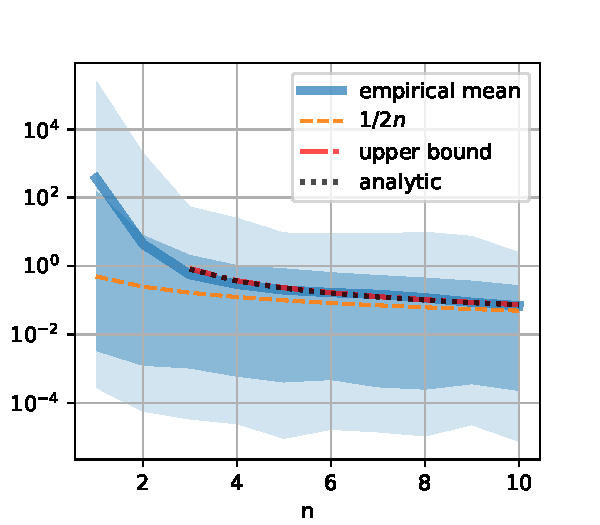
\includegraphics[width=.4\textwidth]{fewsamples.pdf}
	\caption{KL divergence~\eqref{eq:suboptimalityKL} for Gaussian variance MLE (\S\ref{ssec:gaussian-variance}) against number of samples $n$. Bold curve is an average over 10000 trials,  dark shaded area is 90\% confidence interval, light shade is min-max interval. 
		The expected value is infinite for $n=1$ and $n=2$, but for $n\geq3$ it quickly joins the upper bound~\eqref{eq:MLE_rate} and the $1/2n$ asymptote~\eqref{eq:asymptote}, while the variance remains large.
		We wish to find similar upper bounds for a variety of exponential families.
	}
	\label{fig:curves}
\end{figure}


\section{Introduction}
\label{sec:motivation}

{\bf Exponential families} are among the most widely used statistical models.
Many standard random variables fall into this category: Gaussians, categorical, Gamma or Dirichlet.
They are flexible enough to model a variety of data sources $X$, and easy to describe with some sufficient statistics $T(X) \in \real^d$.
In particular, they are appreciated for their convex log-likelihood
\alignn{
f(\nat) = \E[-\log p_\nat(X)] = \logpart(\nat) - \lin{\E[T(X)] , \nat},
\label{eq:defNLL}
}
where $\logpart$ is a convex function and $\nat\in\Theta$ is a vector called \textit{natural parameter}.
This convexity lays the foundation for generalized linear models \citep{mccullagh1989generalized}
or variants of principal component analysis \citep{collins2001generalization}, among other applications.

{\bf Estimators.}
In general, we want to estimate $\nat$ from some data $\mD = (x_1, \dots, x_n)$.
For this purpose, not only is $f$ convex, but it even enjoys a closed form maximum-likelihood estimate (MLE)
\begin{align}
	\nabla \logpart(\hat \nat_n^\text{MLE}) = \frac{\sum_{i=1}^n T(x_i)}{n} \; .
	\label{eq:defMLE}
\end{align}
This rule is known as moment matching.
Given a certain conjugate prior, a similar formula~\eqref{eq:defMAP} holds for the maximum a posteriori (MAP).
The parameter $\theta$ can also be estimated with online-learning techniques, but they are less efficient than offline methods \citep{azoury2001relative,dasgupta2007online}.

{\bf Metrics.}
Once we have an estimator $\hat \nat$, we wish to assess its quality, i.e., its closeness to some optimal $\nat^*$.
This is necessary, for instance to choose between 2 estimators (model selection).
We distinguish here two ways: \textit{disntance in parameter space} and \textit{distance between distributions}.
{\bf 1)} Distance in parameter space $d(\nat,\nat^*)$. This is the focus of \emph{parameter estimation}, yielding results such as the asymptotic efficiency of the MLE via the Cramer-Rao lower-bound \citep{aitken1942estimation} and a wealth of asymptotic results \citep{vdv1998asymptotic}.
In particular for sum of independent variables such as~\eqref{eq:defMLE}, large deviations theory \citep{varadhan1984large} characterizes concentration phenomena.
{\bf 2)} Distance between distributions, as studied in \emph{density estimation}.
For this purpose, the Kullback-Leibler (KL) divergence $\KL\paren{p_{\nat^*} || p_{\nat} }$  arises naturally from information theory,
but its lack of robustness to misspecification\footnote{
For $p$ and $q$ continuous densities,
$\KL(p||q) = +\infty$ if $\exists x, q(x)=0 \&p(x)>0$. 
%Since exponential families have a positive density over their whole input set, this is not a concern for us, except if we misspecified the input set.
}
has led statisticians to study symmetric, better-behaved distances, such as the $L^2$ norm \citep[\S1.2]{tsybakov2009introduction}, the $L^1$ norm \citep{devroye2001combinatorial} or more recently the Hellinger distance \citep{baraud2017new}.
With exponential families, the KL divergence is also a Bregman divergence between parameters (see \S\ref{sec:problem}), thus drawing a connection between these two lines of research.
Hence the fundamental problem:
%\begin{center}
%	\framebox{
%		\parbox[c][]{0.9\linewidth}{
%			\begin{center}
%			\emph{Can we upper bound  the expected value of the KL divergence for MLE or MAP?}
%		\end{center}
%		}
%	}
%\end{center}
\begin{equation}
\boxed{
\begin{aligned}
	\textit{Find an upper}&\textit{ bound on the expected value of } \\
	&\KL(p_{\nat^*} || p_{\hat \nat_n^\text{MLE/MAP} }) \; .
\end{aligned}
}
\tag{$\star$}
\label{problem}
\end{equation}
% RLP : that is a dirty hack, but I would like to be able to reference the problem somehow.

We have already asymptotic solutions (\S\ref{ssec:asymptote}) when $\logpart$ is quadratic (e.g. $X$ is Gaussian with known variance)
or close to quadratic (\S\ref{ssec:quadratic}).
However, a  general solution for finite $n$ remains elusive.
In this paper, we review partial solutions, and give ideas on how to solve it.

{\bf Stochastic optimization} offers an interesting perspective on this question.
Consider the problem
\alignn{
	\min_{\theta\in \Theta} f(\theta)\,,
	\label{eq:optimization_problem}
}
solved by $\nat^*\in \Theta$.
Setting $f$ as the log-likelihood~\eqref{eq:defNLL}, the suboptimality is equal to the KL:
\alignn{
	f(\nat) - f(\nat^*) = \KL\paren{p_{\nat^*} || p_{\nat} }
	\label{eq:suboptimalityKL}
}
Both MLE and MAP can be seen as stochastic algorithms solving~\eqref{eq:optimization_problem}.
In particular, with exponential families, MAP is an instantiation of stochastic mirror descent (SMD) \citep{nemirovski2009robust}.
Inspired by recent work~\citep{lepriol2021analysis, kunstner2020homeomorphic}, we try using existing optimization convergence rates for SMD to get the upper bound we seek.
Unfortunately, none of the current analyses apply, which frames another open problem for the analysis of SMD.

{\bf Expected Ouctomes.}
A solution to~\eqref{problem} would quantify the importance of the prior in MAP, in particular in the few sample regime.%, for instance for Gaussians $\cN(m,\sigma^2)$. 
Also, it could enable stochastic optimization to tackle a wide class of barrier objectives\footnote{we call \emph{barrier} an objective $f$ that is infinite on the boundaries of its domain (assuming they exist).}.
A good example would be generalized linear model based on Gaussians with unknown mean and variance, for which there is currently no theory \citep{bach2013nonstronglyconvex}.
It could also help in assessing the impact of alternative forms of regularization (prior) for these models. 

{\bf Contributions.}
After formalizing the problem~\eqref{problem} (\S\ref{sec:problem}), along with its asymptotic properties (\S\ref{ssec:asymptote}), we make the following contributions.
\begin{itemize}
	\itemsep0em
	\item We provide an upper bound on the KL in the special case of a Gaussian with known mean but unknown variance $\cN(0,\sigma^2)$ (\S\ref{ssec:gaussian-variance}) .
	\item We highlight sufficient conditions to characterize when a (local) quadratic approximation of the KL is valid, offering a partial answer to~\eqref{problem} (\S\ref{ssec:quadratic}-\ref{ssec:local-quadratic}).
	\item We leverage a generalized bias-variance decomposition of Bregman divergences\citep{pfau2013generalized}  to formulate a conjecture about~\eqref{problem}(\S\ref{ssec:bias-variance}).
	\item By linking MAP and SMD, we show modern analysis of SMD are yet to prove convergence on barrier objectives such as $-\log$ (\S\ref{sec:optimization}).
\end{itemize}


{\bf Notation.}
$X$ and $T=T(X)$ are random variables, $x$ is a sample, $n$ is the number of samples and $d= \dim(T)$.
$\langle \cdot , \cdot \rangle$ is the Euclidean scalar product in $\real^d$.


\section{Technical background}
\label{sec:background}
In this section, we review the formalism of exponential families, their duality, a conjugate prior and the corresponding MAP.
We point the reader towards \citet[Chapter 3]{wainwright2008graphical} for a more exhaustive introduction.


The density of an exponential family for a sample $x$ is
\begin{equation}
	 p_\nat(x) = p(x|\nat) = \exp( \langle \nat, T(x) \rangle - \logpart(\nat)) \; ,
	 \label{eq:def_expfamily}
\end{equation}
where  $\nat$ is called natural (or primal) parameter.
It is fully specified by 1) $T: \cX \rightarrow \real^d$, the sufficient statistic,
and 2) a base measure $\nu$ on $\cX$.
Since the exponential is positive, $p$ has the same support as $\nu$.
The log-partition function $\logpart$ acts as a normalization term, since
\begin{align}
    \logpart(\nat) = \log \int e^{\langle \nat, T(x) \rangle} \nu(dx) \;.
\end{align}
This simple model encompasses both categorical distributions : $\cX = \{1, \dots, k\}$, $\nu$ uniform and $T(X)$  the one-hot encoding, and multivariate normal distributions $\cX=\real, \nu$ Lebesgues and $T(X)=(X, X^2)$.

For convenience, we focus on steep, regular exponential families with minimal statistic $T$ \citep{barndoffnielsen2014information}.
Then $\logpart$ is a strictly convex function of Legendre type,
and the set $\Theta = \{ \nat \cond \logpart(\nat) < \infty\}$ is open and convex.
When explicit, we write the random variable $T = T(X)$.

% TODO sort out relationships between : steep family, minimal statistics and Legendre type. What implies what ?

{\bf Duality.}
The log-partition function $\logpart$ verifies the two following identities:
\begin{align}
    \nabla\logpart(\nat) &=  \expect[p_\nat]{T(X)} =: \meanp, \\
    \nabla^2 \logpart(\nat) &= \Cov_{p_\nat}[T(X)] > 0,
\end{align}
where $\meanp$ is called the mean (or dual) parameter, which lives in the open convex set $\cM$ equal to the relative interior of the convex hull of $T(\cX)$.
Given that $\logpart$ is strictly convex, its Hessian is positive definite and its gradient $\nabla \logpart$ is a \textit{bijection} between natural parameters $\nat$ and mean parameters $\m$.
We will write interchangeably $\m$ or  $\nat$ depending on the context, being aware that both are linked and represent the same distribution.

We now introduce the convex conjugate (the Fenchel-Legendre transform) of the log-partition function
\begin{align}
	\conj(\m) =  \langle \m, \nat \rangle - \logpart(\nat)
	=  \max_{\nat'\in\Theta}  \langle \m, \nat' \rangle - \logpart(\nat')\; ,
\end{align}
which is the common notion of \textit{entropy} in information theory.
By Fenchel duality, its gradient is the inverse of the gradient of $\logpart$,  $\nabla\conj=\nabla\logpart^{-1}$, giving
\aligns{
	\nabla\conj \circ \nabla\logpart(\nat) = \nat, \quad \nabla\logpart\circ \nabla\conj(\meanp) = \meanp.
}
%\begin{figure}[t]
%	\centering
%	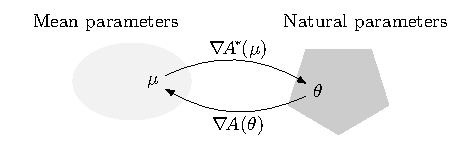
\includegraphics{duality}
%	\caption{The gradient of the log-partition function and its dual, $(\nabla \logpart, \nabla \conj)$, form a bijection between natural and mean parameters $\nat, \meanp$. Figure copied from \citet{kunstner2020homeomorphic}. % TODO make an original one.
%	}
%	\label{fig:duality}
%\end{figure}%
%
%Not super convinced about introducing that here? it comes naturally when considering the KL on exponential maps) %RLP it is useful to the conjugate prior.
{\bf The Bregman Divergence} induced by $\logpart$ measures the discrepancy between two parameters $\nat$ and $\nat_0$,
\begin{align}
    \bregman (\nat ; \nat_0)
    & = \logpart(\nat) - \logpart(\nat_0)
    - \langle \nabla \logpart(\nat_0)  , \nat - \nat_0 \rangle,
    \label{eq:defBregman}
\end{align}
with $\nabla \logpart(\nat_0) = \expect[\nat_0]{T(X)} =: \meanp_0$ the mean parameter associated to $\nat_0$.
In general, Bregman divergences are not symmetric, i.e., $\bregman (\nat ; \nat_0)\neq \bregman (\nat_0 ; \nat)$.
%Finally, it is equal to the divergence of its convex conjugate with switched arguments,
%\begin{align}
%	\bregman (\nat ; \nat_0)
%    = \bregmanconj ( \meanp_0 ; \meanp) \; .
%    \label{eq:bregman_switch}
%\end{align}

{\bf A Conjugate Prior} for $p(X|\nat)$ is
\begin{align}
    p(\nat)
    &\propto \exp( - n_0 \bregman(\nat ; \nat_0) ) \\
    &\propto \exp(n_0 \langle \m_0, \nat \rangle - n_0 \logpart(\nat)),
    \label{eq:def_prior}
\end{align}
where $n_0$ and $\nat_0$ are (hyper)parameters of the prior  \citep{agarwal2010geometric}.
This is an exponential family with sufficient statistics $(\nat ,\logpart(\nat))$ and natural parameter $(n_0 \m_0, -n_0)$.
Intuitively, $n_0$ is the number of fictive data points observed from a distribution with natural parameter $\nat_0$.

{\bf Maximum A Posteriori (MAP)}
Given a dataset $\mD_n =(X_1,\dots,X_n)$, we wish to estimate the maximum of the posterior distribution $p(\nat \cond \mD_n) \propto p(\mD_n|\nat)p(\nat)$.
Plugging in~\eqref{eq:def_expfamily},~\eqref{eq:defBregman} and~\eqref{eq:def_prior} yields
\begin{align}
	p(\nat \cond \mD_n)
    \propto \exp(- (n_0+n) \bregman(\nat; \MAPt^\text{MAP}))
    \label{eq:joint_likelihood}
\end{align}
which reaches its maximum at $\MAPt^\text{MAP}$ such that
\begin{align}
    \nabla \logpart(\MAPt^\text{MAP}) = \MAPm^\text{MAP}
    = \frac{n_0 \meanp_0 + \sum_{i=1}^n T_i}{n_0+n} \; ,
    \label{eq:defMAP}
\end{align}
where $T_i=T(X_i)$.
When $n_0=0$ (no samples from the prior), we recover the MLE~\eqref{eq:defMLE}.
We write $\MAPt$ for the MAP, and view the MLE as a special case.


\section{PROBLEMS FORMULATION}
\label{sec:problem}
% Assume we observe a dataset $\mD$ drawn i.i.d. from a distribution $\cD$.
% We further assume that our model is well-specified and there exist $\nat^*\in\Theta$ such that $\cD = p(\cdot \cond \nat)$.
% As we will see, this is already an interesting setting.
% We wish to estimate how well the MLE or a MAP model the true distribution.

We are now ready to formalize the main problem of this paper. Assume we observe a dataset $\mD$ drawn i.i.d. from $p(\cdot \cond\nat^*)$, an exponential family distribution
with parameters $\nat^*$.
We wish to quantify how well the MLE or a MAP models the true distribution.

A natural way to quantify this is the Kullback-Leibler divergence (KL) $\KL(p_{\nat^*} || p_\nat)$. % should we define it ?
In the well-specified setting it corresponds to the log-likelihood sub-optimality~\eqref{eq:suboptimalityKL}.
With exponential families, the KL is also a Bregman divergence:
\alignn{
	\KL(p_{\nat^*} || p_\nat)
	 = \bregman(\nat ; \nat^*)
	 = \bregmanconj(\m^* ; \m) \; .
}
The second equality is a general property of Bregman divergences and convex conjugates. % (Be careful about the order of arguments.)
How does this quantity behave when $\nat$ is the MLE or MAP?
 Or in the words of statistical decision theory, what is the \emph{frequentist risk} of these estimators when the loss is the KL divergence? 
This is our first problem.

\begin{problem}[Upper-bounding MAP and MLE]
Upper bound the following quantities:
\begin{align}
	\label{eq:bregmanMLE}
	\text{MLE: } \quad &\expect[\mD]{\bregmanconj \left (\E [T] ;  \inv{n}  \smallsum_i T_i \right )}, \\
	\label{eq:bregmanMAP}
	\text{MAP: } \quad &\expect[\mD]{\bregmanconj \left (\E [T] ; \frac{n_0 \m_0 + \smallsum_i T_i}{n_0+n} \right )},
\end{align}
where the expectation is on the data $\mD = (T_1, \dots, T_n)$.
\end{problem}

More explicitly, we want an upper bound that does not involve this expectation over the dataset.
Surprisingly, we found no general solution to this seemingly simple problem, whether in the literature or by our own means.
In \S\ref{sec:example}, we provide results for special cases such as $\cN(0, \sigma^2)$,
while in \S\ref{sec:insights} we provide realistic conditions to obtain bounds that are valid after seeing a large number of samples.
But we are yet to find a solution encompassing both a broad range of exponential families,
and applicable to small sample sizes $n \lesssim d$.

{\bf A Difficulty with the MLE.}
While~\eqref{eq:bregmanMAP} is always finite, \eqref{eq:bregmanMLE} may be infinite,
for instance when estimating the covariance of a Gaussian when $n \leq d + 1$.
Even worse, with categorical variables, there is a non-zero probability to never sample one of the categories.
In those cases the MLE gives zero weight to this category and $\KL(p_{\nat^*} \,\Vert\, p_\text{MLE} ) = +\infty$.
Therefore, the expected KL~\eqref{eq:bregmanMLE} is infinite for any number of samples.
Instead of taking the expectation, one might want to bound the risk in high probability,
without resorting to Markov inequality but this is a difficult endeavor.
These examples make a case for regularized estimators such as MAP,
for which we may find upper bounds.

\paragraph{Optimization}
With exponential families, MAP can be seen as \emph{an instantiation of stochastic mirror descent (SMD).}
More precisely, let us re-write~\eqref{eq:defMAP} as
\alignn{
\m_n = \m_{n-1}- \lr_n (\m_{n-1} - T_n)
\label{eq:mean_update}
}
where $\lr_n := \inv{n_0 + n}$.
Now define stochastic functions $f_X(\nat) = -\log p(X \cond \nat)$ such that $\E[f_X] = f$.
If we further introduce stochastic gradients $g_n(\nat) := \nabla\logpart(\nat) - T_n = \nabla f_{X_n}(\nat)$, then~\eqref{eq:mean_update} becomes
\alignn{
	\nabla\conj(\hat \nat_{n})
	= \nabla\conj(\hat \nat_{n-1}) - \lr_n g_n(\hat \nat_{n-1}),
}
which is the update formula for SMD on $f$ with mirror map $\nabla\logpart$
and step-size schedule $\lr_n$, initialized at $\nat_0$.
In this view, MLE forgets its (arbitrary) initialization after the first step with step-size 1.	
The observation MAP$\in$SMD brings us to our second problem.
\begin{problem}[Convergence rate for SMD]
Find a convergence rate for stochastic mirror descent that applies to conjugate MAP of exponential families such as Gaussians $\cN(\meanp, \sigma^2)$.
\end{problem}

To address these problems, we start by investigating examples, for which we provide solutions to problem 1 and get insights into what is achievable.

\section{Examples}\label{sec:example}
\subsection{Gaussian Variance}\label{ssec:gaussian-variance}

A simple yet non-trivial example is the centered Gaussian distribution with unknown variance $\cN(0,\sigma^2)$.
Its log-likelihood reads $\log p(x) = -\frac{x^2}{2 \sigma^2} - \half\log(2\pi \sigma^2)$.
Defining $T(X)=X^2$ as the sufficient statistic, we get natural parameter $\nat = -\inv{2 \sigma^2} <0$, and mean parameter $\m=\E[T(X)] = \sigma^2 >0$.
Mean and natural parameters are roughly inverse of each other, i.e., $\nat = -\inv{2 \m}$.
\textcolor{red}{The explanation here is not clear enough, or too concise} 
Now we can match the log-likelihood with the exponential family template to get the log-partition function, and take the conjugate to find the entropy
\aligns{
	\logpart (\nat) = - \half \log(-\nat) \quad\text{and}\quad
	\conj(\m) = - \half \log(\m)  \; ,
}
up to constants.
Both the log-partition and  the entropy are roughly negative logarithm $z\mapsto - \log(z)$.
It means the conjugate prior is the exponential family with sufficient statistic $(\nat, \log(-\nat) )$, e.g., a negative Gamma distribution.
It also means $\bregman$ and $\bregmanconj$ have the same shape
\begin{align}
	\bregmanconj( \m_*; \m_n)
	&= \half \left ( \frac{\m_*}{ \m_n} - 1 - \log  \frac{\m_*}{ \m_n} \right), \\
	\bregman( \nat_n; \nat_* )
	&=  \half \left ( \frac{ \nat_n}{\nat_*} - 1 - \log  \frac{ \nat_n}{\nat_*} \right) \; .
\end{align}
In theorems~\ref{thm:varianceMLE} and~\ref{thm:varianceMAP}, we report upper bounds on the expected value of this divergence for the MLE and the MAP.
All proofs for this section are in \cref{app:gaussian-variance}.
\begin{theorem}[MLE Bound]
\label{thm:varianceMLE}
	The MLE of $\cN(0,\m_*)$ is $\hat \m_n^\text{MLE} = \inv{n} \sum_i X_i^2 $.
	Its expected suboptimality is infinite when $n\leq 2$, and otherwise upper-bounded as
	\begin{align}
		 \expect{\bregmanconj( \m_*; \hat \m_n^\text{MLE}) }
			\leq \inv{2n} +\frac{2}{n(n-2)} \; .
			\label{eq:MLE_rate}
	\end{align}
\end{theorem}
This upper bound matches the asymptote~\eqref{eq:asymptote} .
We illustrate its numerical behavior in Figure~\ref{fig:curves}.
With the same technique, we obtain a similar bound for the multivariate generalization: the expected value is infinite whenever $n \leq d+1$ where $d$ is the dimension, and is otherwise bounded by $O(\frac{d^2}{n} + \frac{d^3}{n(n-d-1)} )$.

\begin{theorem}[MAP Bound]
\label{thm:varianceMAP}
The expected suboptimality of the MAP of $\cN(0,\m^*)$ with prior hyper-parameters $(n_0,\m_0)$ is
 \begin{align}
	& \expect{\bregmanconj( \m_*; \hat \m_n^\mathrm{MAP})}
	\leq \begin{cases}
		\inv{2(n_0+1)}  +  b_1 \ \text{if}\ n=1,\\
		\frac{1}{n_0 \frac{\m_0}{\m^*} +n-2} + b_n \ \text{if}\ n\geq 2
	\end{cases}
	\label{eq:MAP_rate}\\
	& \text{where }b_n = \frac{(1 + \inv{n_0} - \frac{\m_0}{\m^*})^2}{2 (\frac{\m_0}{\m^*}+\frac{\max(0,n-2)}{n_0})(1 + \frac{n}{n_0} )} \; . \nonumber
\end{align}
\end{theorem}
Note that this inequality actually holds for the symmetrized Bregman $\cB(a,b) + \cB(b,a)$, which explains why it loses a factor 2 compared to the asymptote~\eqref{eq:asymptote}, but we leave this to the appendix for clarity.
Anticipating on \S\ref{ssec:bias-variance}, this inequality highlights a clear variance-bias decomposition.
In particular, there is no bias term when $\frac{\m_0}{\m^*} =1 + \inv{n_0} $, which happens when the prior is slightly larger than the ground truth
This correlates well with our numerical observations (cf App.\ref{app:gaussian-variance}).

\begin{figure*}[t]
	\centering
	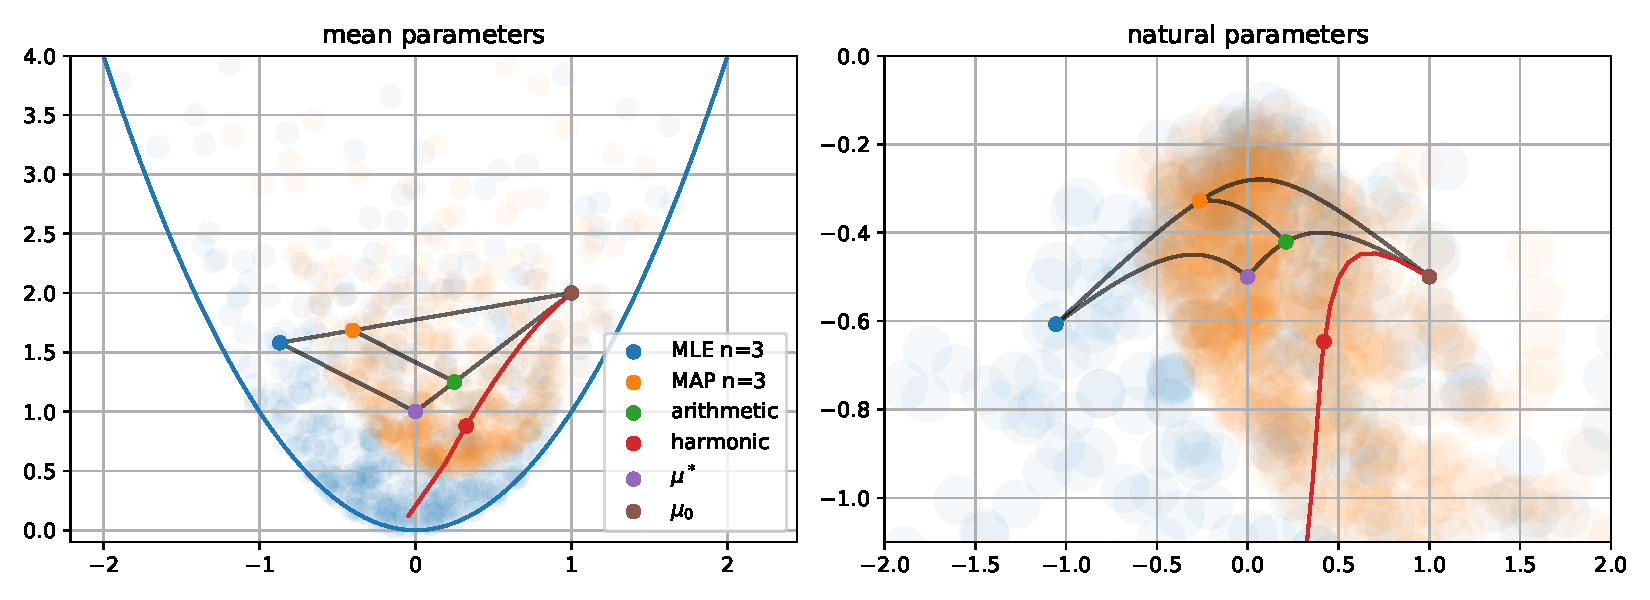
\includegraphics[width=\textwidth]{figs/thales/numerical_schema_n=3.pdf}
	\caption{A numerical illustration of the different characters featured in the bias-variance decomposition, for a 1D Gaussian $\cN(\mu, \sigma^2)$.
	}
	\label{fig:thales}
\end{figure*}

\subsection{Gaussian}
\label{ssec:gaussian}
Now that we have solved the case of $\cN(0,\sigma^2)$, let's move on to the ubiquitous Gaussian $\cN(m,\sigma^2)$.
Gaussians actually offers a highly non-trivial example for Problem 1.
Their log-likelihood reads $p(x) = -\frac{(x-m)^2}{2 \sigma^2} - \half \log(2\pi\sigma^2)$.
With sufficient statistic $T(x)=(x, x^2)$, 
the mean parameters are $\m = \E[T(X)] = (m , m^2 + \sigma^2)$ belonging to the open set $\cM= \{(u,v) \cond u^2 < v\}$,
and the natural parameters are $\nat= (\frac{m}{\sigma^2} , \frac{-1}{2\sigma^2}) \in \Theta = \real \times \real_-$. 
Examples of MAP and MLE  are represented in \cref{fig:thales} within $\cM$ and $\Theta$ delimited in grey.
Given these parameters, log-partition and entropy are, up to constants, 
\alignn{
	\logpart(\nat) &= \frac{\nat_1^2}{-4\nat_2} - \half \log(-2\nat_2) \\
	\conj(\m) &= - \half \log (\mu_2 - \mu_1^2)
}

These functions are neither smooth, nor strongly convex, nor self-concordant (see \cref{app:gaussian}).
Let us keep this in mind, as we move on to discussing the general problem, and some ways to solve it via direct expansions of the Bregman divergence.

\section{Partial Solutions}
\label{sec:insights}

\subsection{Asymptote}
\label{ssec:asymptote}
As a reference point for any finite convergence rate, it is interesting to know the asymptotic behavior of these quantities as $n \rightarrow +\infty$.
We now review classical asymptotic results.
We point the reader towards \citet[\S1.1]{ostrovskii2021finite} for a more comprehensive overview.
Asymptotic results typically show that the MLE expressed with natural parameters $\nat$ is asymptotically normal: it reaches the Cramér-Rao lower bound \citep[for instance Ch4.2]{vdv1998asymptotic}.
With exponential families, the MAP is more simply expressed with mean parameters $\meanp$.
We get the asymptote by approximating the Bregman divergence using a second order Taylor expansion
\alignn{
    \bregmanconj(\m^* ; \m)
    &= \frac{\norm{\m^* - \m}^2_{\mF}}{2}
    + O(\norm{\m - \m^*}^3),
    \label{eq:bregmanTaylor}
}
where the Mahalanobis norm  $\| x \|_{\mF}^2 = x^\top \mF x$  is induced by $\mF  := \nabla^2\conj(\m^*)$, the hessian of the entropy at the optimum. It happens that  $\mF$ is also the inverse \textit{Fisher information matrix} at $\nat^*$, since
\aligns{
    \mF
    :=\nabla^2\conj(\m^*)
    = \nabla^2\logpart(\nat^*)^{-1}
    = \Cov_{\nat^*}[T(X)]^{-1}  \; .
}
Plugging~\eqref{eq:defMLE} or~\eqref{eq:defMAP} into~\eqref{eq:bregmanTaylor}, one can show that MLE and MAP verify
\begin{align}
	\label{eq:asymptote}
	\E \bregmanconj \left (\E [T(X)] ; \hat \meanp_n^\text{MLE/MAP} \right )
	= \frac{d}{2n} + O(n^{- \frac{3}{2}}) \; .
\end{align}
Detailed derivation is in~\cref{app:asymptote}
Both MLE and MAP have the same asymptote, as the contribution of the prior $n_0 \meanp_0$ gets negligible compared to the data for large $n$.
This asymptote is also independent of the optimum $\meanp^*$.

\subsection{Quadratic Case}
\label{ssec:quadratic}
As another classical reference point, let us consider the case $\logpart(\nat) = \half \norm{\nat}_2^2$.
For instance, this is the log-partition of a Gaussian with known variance $I$,
\[
	\cX=\real^d,\quad \nu(dx) = \exp\paren{\textstyle \half[-\|x\|^2]} dx,\quad T(x)=x.
\]
Then $\conj(\meanp) = \half \norm{\meanp}_2^2$ as well, and both Bregman divergences are squared $\ell^2$ distances:
\begin{align}
	\bregmanconj(\meanp^* ; \meanp) = \half \norm{\meanp^* -  \meanp }_2^2  \; .
\end{align}
Thanks to the independence of samples, we can break down the MLE into individual point's contributions
\begin{align}
	\expect{\half \norm{\m^* -  \inv{n}  \smallsum_i T_i}_2^2}
	=\frac{\Var(T)}{2n}
	=\frac{1}{2n}
\end{align}
Adding a reference mean $\m_0$ to get the MAP yields to
\begin{align}
	\expect{\bregmanconj(\meanp^*; \MAPm)}
	&= \frac{n \Var(T) +  n_0^2 \norm{\m^* -  \m_0}^2}{2(n+n_0)^2}.
	%\\ &= O\left(\frac{\Var(T)}{n} \right) + O\left(\frac{\norm{\m^* -  \m_0}^2}{n^2} \right)
	\label{eq:MAP_quadratic}
\end{align}
In both cases, we have a variance term in $O(n^{-1})$ and a bias term in $O(n^{-2})$. Ideally, such result should also similarly for arbitrary exponential families.
If we make restrictive assumptions on the log-partition function, we can relate $\bregmanconj$ to a norm or a quadratic.

{\bf If $\conj$ is $L$-Lipschitz} (e.g. $\logpart$ is defined within the $\ell^2$-ball of radius $L$), then
\begin{align}
    \bregmanconj(\m^* ; \m)
    &\leq L \norm{\m^* - \m} + \norm{\nat} \norm{\m^* - \m} \\
    &\leq 2L \norm{\m^* - \m}
\end{align}
so $\bregmanconj$ is $2L$-Lipschitz, and we get a $O(\inv{\sqrt{n}})$ rate.
Note that none of the standard exponential families verify this assumption.
\TODO{connection with optim non-smooth rate.}

{\bf If $\conj$ is $L$-smooth}\footnote{e.g. $\nabla\conj$ is $L$-Lipschitz.} (e.g. $\logpart$ is $\frac{1}{L}$-strongly convex \citep{kakade2009duality}), then
\begin{align}
    \bregmanconj(\m^* ; \m)
    \leq \frac{L}{2} \norm{\m^* - \m}^2
\end{align}
so $\bregmanconj$ is upper bounded by a quadratic, and we get~\eqref{eq:MAP_quadratic} as an upper bound.
Besides the Gaussian with known variance, no standard exponential family verify this assumption either.
Note that it is also possible to get (more complex) upper bounds under restricted notions of strong-convexity \citep{negahban2012unified}.
\TODO{connection with optim smooth rate.}

\subsection{Locally Quadratic Case}
\label{ssec:local-quadratic}
FromTaylor expansion~~\eqref{eq:bregmanTaylor},
we know that all Bregman divergences are locally quadratic.
Under some assumptions, such as self-concordance of $\conj$\footnote{
In 1d, $f$ is self-concordant iff $\forall x, \abs{f'''(x)} \leq 2 \abs{f''(x)}^{\frac{3}{2}}$.
} \citep[Ch.4.1]{nesterov2003introductory}, we can quantify when this quadratic behavior kicks in. Proofs for this subsection are in \cref{app:self-concordant}.
\begin{proposition}
Let $\conj:\cM\rightarrow \real$ be a self-concordant convex function, $\m, \m^* \in\cM$ and $\mF = \nabla \conj(\m^*)$. Then
\aligns{
	\norm{\m^*-\m}_{\mF} < 0.21
	\implies
	\bregmanconj(\m^*,\m) \leq \norm{\m^*-\m}_{\mF}^2
}
\end{proposition}
\footnote{$0.21$ is a value of $x$ such that $x^2 \geq -\frac{x}{1-x} - \log(1 - \frac{x}{1-x})$}.
To gain insights into how many samples are needed, we can estimate when $\expecti{\norm{\m^*-\m}_{\mF}} < 0.21 $.
For the MLE, $\expecti{\norm{\m^*-\hat \m_n}_{\mF}} = \frac{d}{n}$, so a sufficient condition is $n \geq 5 d$.
For MAP, using~\eqref{eq:MAP_quadratic}, we get the sufficient condition $n\geq 5d + \sqrt{5}\norm{\m^* -  \m_0} - n_0$.
This means that on average, we need much more samples than the dimension to reach the quadratic regime.

We know that $\conj$ is self-concordant when $T$ is 1-dimensional and $\logpart$ is self-concordant.
This is true for
exponential distributions,
Gaussians with known mean,
Laplace with known mean,
Pareto with known minimum value,
or Weibull with known shape $k$.
The entropy is also self-concordant when $T$ lives in a compact \citep{bubeck2015entropic}.
This is true for categorical or Dirichlet distributions.

With some more work, it is possible to get a wealth of results under this assumption.
For instance \citet{ostrovskii2021finite} characterizes the number of samples needed to reach this quadratic behavior for arbitrary parametric models, under the assumptions of self-concordance, or pseudo self-concordance \citep{bach2010self}.
Or in the world of exponential families, \citet{kakade2010learning} assumes a local bound on all higher order moments of $\logpart$ in $\nat^*$, to quantify when $\logpart$ can be sandwiched between quadratics in $\nat$, but this does not directly translate into quadratics in $\m$.

All these works give \textit{large sample} results -- results that hold only for $n\geq N$ for some constant $N$ -- but none of them  apply to small $n$.


\citet{anastasiou2017bounds} and
\citet{marteauferey2019beyond})
\fdk{
We know that if the problem is strongly convex (in $\norm{\cdot}_2$), averaged SGD achieves $O(1/n)$ rate.
[Robust stochastic approximation approach to stochastic programming]. (The paper uses a bounded stochastic gradient assumption, but can be relaxed to bounded variance instead.) However, strong-convexity in the Euclidean norm is not strictly necessary to find an algorithm with convergence rate of $O(1/n)$, as shown by [Non-strongly-convex smooth stochastic approximation with convergence rate O(1/n)] for linear and logistic regression. Their proof techniques based on self-concordance have been extended to other setting, [Finite-sample analysis of M-estimators using self-concordance, Learning Exponential Families in High-Dimensions: Strong Convexity and Sparsity].
The same tools are used in statistics, and evething essentially boils down to controlling how different we are from a Gaussian rv, that we're going to get by the CLT, like [Bounds for the normal approximation of the maximum likelihood estimator, Anastasiou].
}

\subsection{Bias-Variance Decomposition}
\label{ssec:bias-variance}
In both the quadratic~\eqref{eq:MAP_quadratic} and the Gaussiance variance examples~\eqref{eq:MAP_rate}, the upper bound takes the form $O(\inv{n}) + O(\frac{\text{bias}}{n^2})$, 
giving us a flavor of what we would like as a general result for exponential families : a finite sample convergence rate, with a variance and a bias terms that reflect the important constants of the problem.
In fact, such a decomposition exists for any Bregman divergence.
Let $\tilde \theta_n := \expecti{\hat \theta_n}$ be the expectation of the MAP in primal space, and $\tilde \m_n = \nabla \logpart(\tilde \theta_n )$ be its corresponding mean parameter.
As described by \citet[Theorem 0.1]{pfau2013generalized}, the  expected Bregman decomposes into
\begin{equation}
	\expect{\bregmanconj(\m^* ; \hat \m_n)} = {\bregmanconj(\m^* ; \tilde \m_n)}
	+ {\expect{\bregmanconj(\tilde \m_n ; \MAPm)}}
	\label{eq:primal_pivot}
\end{equation}


\textbf{Remark:} In this decomposition, the primal expectation $\expect{\hat \theta_n}$ is taking the role of pivot / reference point. An estimator will be unbiased if its primal expectation is non-zero.
However, this is not true for the the gaussian variance MLE, where the bias decreases like ${\bregmanconj(\m^* ; \tilde \m_n)} \leq \frac{2}{n(n-2)}$.
A contrario, the MLE is unbiased wrt the dual parameter, but the decomposition there is not clean.

\textbf{Conjecture:} the bias decreases like $O(1/n^2)$.

\paragraph{Illustrations.}
We plot the bias-variance decompositions for $\cN(0,\sigma^2)$ (Figure~\ref{fig:variance_decomposition}) and  $\cN(\mu, \sigma^2)$ (Figure~\ref{fig:gaussian_decomposition}).
Additionally,  for $\cN(\mu, \sigma^2)$, Figure~\ref{fig:thales} plots the characters featured in these decompositions $\hat \m_n^\text{MLE},\hat \m_n^\text{MAP},\m_n,\tilde \m_n, \m^*$ and $\m_0$ (and corresponding primal parameters) . \rlp{Tune figures.}\textcolor{red}{Not super clear, what is the "characters featured in these decompositions?"}


\begin{figure}[t]
	\centering
	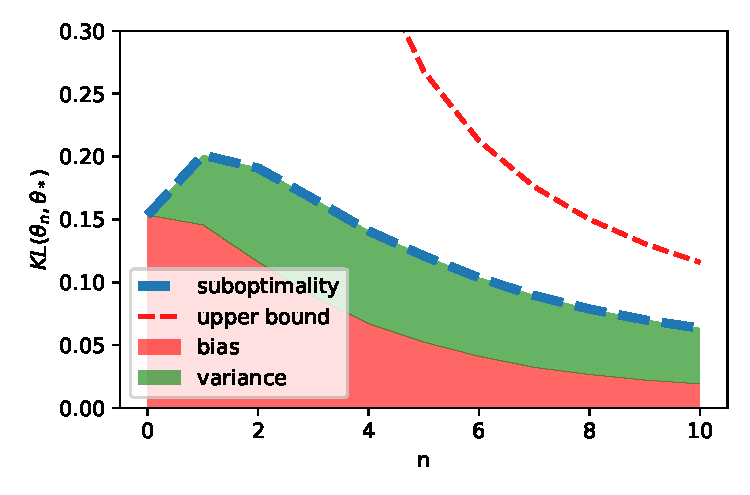
\includegraphics[width=.4\textwidth]{figs/gaussian_variance.pdf}
	\caption{
	\textbf{Gaussian variance $\cN(0,\sigma^2)$ example. Left:} training curves and analytic upper bound.
	\textbf{Center:} bias-mixed-variance decomposition, using the arithmetic mean.
	\textbf{Right:} bias-variance decomposition, using the harmonic mean.
	}
	\label{fig:variance_decomposition}
\end{figure}

\begin{figure}[t]
	\centering
	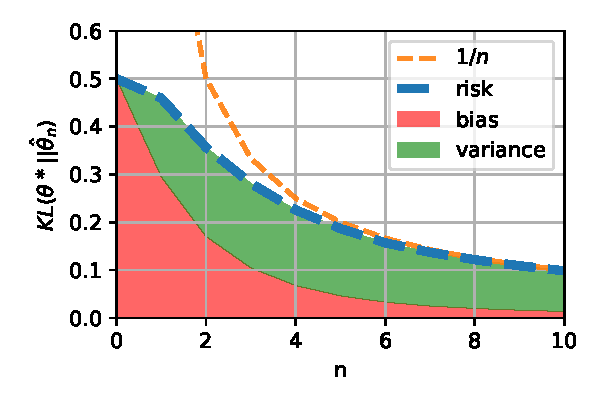
\includegraphics[width=.4\textwidth]{figs/gaussians/new_linear_n0=1.pdf}
	\caption{
	\textbf{Full gaussian} $\cN(m, \sigma^2)$ with $\meanp^*=(0, 1), \meanp_0 = (1,2)$ and $n_0=1$. \textbf{Left:} training curves (5,95) percentiles, average and asymptote.
	\textbf{Right:} bias-variance decomposition.
	}
	\label{fig:gaussian_decomposition}
\end{figure}



\section{AN OPTIMIZATION PROBLEM}
\label{sec:optimization}


%This section show how MAP can be interpreted as stochastic mirror descent (SMD). Thanks to this strong link, we show that \textbf{1)} we may obtain a convergence rate for MAP from the rate od SMD, and \textbf{2)} any insights gained from the MAP may inform on further design and analysis of SMD.
%Then, we review the assumptions of relative smoothness, useful to deal with non-smooth functions, before investigating three different analyses of SMD with the MAP.
%\rlp{mention that examples have so far been lacking for relative SMD.}
%
%\subsection{MAP as Stochastic Mirror Descent}
%\label{ssec:MAP=SMD}
%By the Bayes rule, the posterior can always be written iteratively $p(\nat | \mD_n) \propto p(X_n | \nat) p(\nat | \mD_{n-1})$.
%Plugging in~\eqref{eq:joint_likelihood}, and introducing $f_n(\nat) = - \log p(X_{n} | \nat)$, we see that the MAP verifies
%\begin{align*}
%	\hat \nat_{n}
%	= \argmin_\nat f_n(\nat) + (n_0 + n -1) \bregman(\nat; \hat \nat_{n-1})
%    %\label{eq:SBPP}
%\end{align*}
%which is the update of a Stochastic Bregman Proximal Point update with step-size $\inv{n_0 + n - 1}$.
%%Maybe skip this SBPP story altogether
%If we expand $f_n(\nat) = \logpart(\nat) - T_n$,  we get (after some manipulation with the Bregman divergence)
%\begin{align*}
%		\hat \nat_{n}
%	= \argmin_\nat \langle g_{n}(\hat \nat_{n-1}), \nat \rangle + (n_0 + n) \bregman(\nat; \hat \nat_{n-1})
%    %\label{eq:SMD}
%\end{align*}
%where $g_{n}(\nat) := \nabla f_n(\nat) = \hat \m_{n-1} - T_n$.
%We recognize the update of Stochastic Mirror Descent (a.k.a. Stochastic Bregman Gradient) with step-size $\lr_n = \inv{n_0 + n}$.
%From the first order optimality condition, we see this is a stochastic gradient step in the dual $\hat \m_n = \hat \m_{n-1} - \lr_n g_n$.
%This parallel means we could obtain a finite convergence rate for the  MAP from an analysis of these algorithms.
%In particular, it could potentially apply to a wide range of distribution $\cD$ on $X$.
%Note that this optimization perspective does not hold for the MLE %($n_0=0$)
%as its implicit uniform prior may correspond to an initialization outside of $\Theta$.

As we saw in the technical background, MAP can be interpreted as stochastic mirror descent (SMD).
This means that \textbf{1)} we may obtain a convergence rate for MAP from an optimization analysis, and \textbf{2)} any insights gained from the MAP may inform further design and analysis of SMD.
We first review the assumptions of relative smoothness, useful to deal with non-smooth functions, before investigating 3 analysis of SMD with the MAP.
\rlp{mention that examples have so far been lacking for relative SMD.}

\subsection{Relative Smoothness}
Mirror descent (MD) \citep{nemirovski1983problem,beck2003mirror}, also known as
Bregman (proximal) gradient, relative gradient descent or NoLips,
%Nemirovski introduced the algorithm, and Beck established the connection with Bregman divergences, e.g. the argmin form.
and SMD
\citep{nemirovski2009robust,ghadimi2012optimal}
are typically encountered in non-smooth (online) optimization,
under bounded (or Lipschitz) gradient assumption on the objective $f$
and strong convexity assumption on the potential $\logpart$
\citep[Th.4.2(MD) \& Th.6.3(SMD)]{bubeck2015convex}.
In our case, none of these assumptions may hold.
For instance $\logpart = -\log$ is neither smooth nor strongly convex.

Recently, these assumptions have been relaxed to the $\stgcvx$-strong convexity and $\smooth$-smoothness of $f$
\emph{relative} to $\logpart$, defined as
\aligns{
	\stgcvx \cB_{A}(x, y)
	\leq
	\cB_f(x,y)
	\leq
	\smooth \cB_A(x,y) \; .
}
When $\logpart = \norm{\cdot}^2$, we recover standard (Euclidean) smoothness, and gradient descent.
Those conditions ensure the linear convergence of MD with $A$ as the reference function,
thus extending the theory to a family of non-smooth functions $f$ and non-strongly convex potential $\logpart$
\citep{birnbaum2011distributed, bauschke2017descent, lu2018relatively}.

For exponential families, the log-likelihood perfectly fit into this framework, as
\aligns{
	f(\theta) = A(\theta) - \expect{\lin{X, \theta}}
}
is both $1$-smooth and $1$-strongly convex relative to $A$. 
So we are left with finding an applicable convergence rate for SMD under relative assumptions.
As we investigate in the next section, several pieces of work have addressed this question, under various assumptions on the stochasticity \citep{hanzely2018fastest, dragomir2021fast, dorazio2021stochastic}.

\subsection{Bounding the Randomness}
\TODO{compress this section}

To analyze stochastic algorithms, one also need to quantify the randomness.
Many assumptions exist for SGD \citep[\S3 for a modern review]{khaled2020better}.
We now review attempts at analyzing SMD under relative smoothness assumption, in the light of  the MAP example.
See \cref{tbl:assumptions} for a summary.

\textbf{Caveat :} all of these rates apply to the Bregman in the other direction, e.g. $\bregman(\nat^*, \MAPt)$, and sometimes not on the last iterate, but with tail averaging in the primal.

\begin{table}[t]
\begingroup
%\renewcommand*{\arraystretch}{1.25}%
\newcommand*{\greencmark}{\textcolor{Green}{\cmark}}
\newcommand*{\redxmark}{\textcolor{Red}{\xmark}}
\centering
\caption{Summary of results for SMD
under relative smoothness and relative strong convexity assumptions.
Barrier tells whether the assumption can hold with barrier objectives.
$\lr_n \sim \inv{n}$ says whether the convergence rate hold with this step-size scheduling, and the last column tells whether the rate applies to the last iterate or to some average iterate.
}
\begin{tabular}{lccc}
%{p{.15\textwidth}m{.05\textwidth}m{.08\textwidth}m{.1\textwidth}}
\toprule
Boundedness & Barriers &  $\lr_n \sim \inv{n}$ & Last iterate \\
\midrule
%Strongly convex and bounded variance\newline
%\citep[e.g.,][]{??}
%&
%$
%\cB_A(\theta,\theta') \geq \frac{1}{2}\norm{\theta-\theta'}^2,
%\quad
%\expect[x]{\norm{\m - x}}^2\leq\sigma^2
%$
%\\
Var. on $\Theta$~\eqref{eq:hanzely} % \newline \citep{hanzely2018fastest}
& \redxmark & \greencmark  & \redxmark
\\
Var. at $\theta_*$~\eqref{eq:dragomir} %\newline \citep{dragomir2021fast}
& \redxmark & \greencmark  & \greencmark
\\
Opt. gap~\eqref{eq:dorazio} %\newline \citep{dorazio2021stochastic}
& \greencmark & \redxmark & \greencmark
\\
\bottomrule
\end{tabular}
\label{tbl:assumptions}
\endgroup
\end{table}

\subsubsection{Bounded Variance}
\citet{hanzely2018fastest} assume the covariance between negative gradient and next iterate is upper bounded at every time step: $\forall n \geq 1, \forall \hat \nat_{n-1},$
\alignn{
\Cov(-g_n(\hat \nat_{n-1}) , \MAPt) \leq \lr_n C
\label{eq:hanzely}
}
for some constant $C$.
For a Gaussian with known variance ($A(\theta) = \frac{1}{2}\norm{\theta}^2$),
this definition recovers the variance of the stochastic gradient
\[
	\expect[\tilde g_t\!\!]{\norm{\nabla f(\theta) - \tilde g(\theta)}{}^2}\leq C.
\]
More generally, if $A$ is $\stgcvx$-strongly convex w.r.t. $\norm{\cdot}$,
the LHS of \cref{eq:hanzely} is bounded by
$\expecti{\frac{1}{\stgcvx}\norm{\nabla f(\theta) - \tilde g(\theta)}{}^2_*}$.
Then a bound on the variance of stochastic gradients is sufficient for \cref{eq:hanzely}
to hold.
%Another perspective on this covariance is as the expectation of the symmetrized Bregman $\cS_\conj(\m_1, \m_2) = \bregmanconj(\m_1, \m_2) + \bregmanconj(\m_2, \m_1)$ between stochastic and deterministic updates
%\aligns{
%\Cov(-g_n(\hat \nat_{n-1}) , \MAPt) = \E[\cS(\MAPm - \lr g_n  )]
%}
%thus showing positivity.
Under this assumption, \citet[Lem.4.8]{hanzely2018fastest} prove a $O(1/n)$ convergence rate with a $O(1/n)$ step-size, by applying polynomial tail averaging \citep{lacostejulien2012simpler} in primal space $\Theta$.

In general however, this assumption hardly holds.
For the MAP, this translates into $\forall n \geq 1,$
\alignn{
\expect[T_n]{\lin{T_n - \mu^* , \MAPt}} \leq \lr_n C
}
which fails to hold on the gaussian variance example for instance. \TODO{ DAMIEN short proof or formalize.}

\subsubsection{Bounded Variance at the Minimum}

\citet{dragomir2021fast} introduce a much weaker assumption $\forall n \geq 1, \forall \MAPm,$
\alignn{
	\expect[\tilde g]{
		\cB_{A^*}(\MAPm - 2\lr g(\theta_*), \MAPm)
	} \leq 2 \lr^2 C \; .
	\label{eq:dragomir}
}
In words, this bounds the variance of the gradients at the minimum, but with a metric that depends on the iterate $\MAPm$, and this bound should hold for every iterate we may encounter on the stochastic trajectory.
% As observed by Frederick, this is really weaker than Hanzely, because it is only the first half of their assumption. There is only a factor 2 that's preventing a direct inequality.
Under this assumption, they prove convergence up to a variance ball with a constant step-size.
Their descent lemma \citep[Eq.(12)]{dragomir2021fast} is the exact analog  of a modern analysis of SGD \citep[Th.3.2]{gower2019sgd}, meaning we can plug in a $O(1/n)$ decreasing step-size and obtain a $O(1/n)$ convergence rate.

This seems to be a perfect solution to our problem. Yet it suffers from the exact same qualm as \citet{hanzely2018fastest}. For barrier objectives, \cref{eq:dragomir} cannot hold uniformly on every possible path of iterates, because these paths can get arbitrarily close from boundaries where $\bregmanconj$ becomes infinite.

\subsubsection{Bounded Optimality Gap}
Inspired by \citet{loizou2021stochastic}, \citet{dorazio2021stochastic} explore the hypothesis
\alignn{
\min_\nat f(\nat) - \expect[X]{\min_\nat f_X(\nat)} \leq C,
\label{eq:dorazio}
}
where $f_X$ is a stochastic estimate of $f = \expecti{f_X}$. In our case $f_X(\nat) = - \log p(X\cond \nat)$.
In words, this lower bounds the expectation of the minimum of the stochastic estimates.
For probabilistic models, such a bound is finite as soon as the model cannot give infinite density to any data point $x$.
This holds for instance for discrete distributions because the probability mass is upper bounded by $1$,
but it rules out  many families.
In the case of normal distributions$\cN(m, \sigma^2)$, setting $\mu=x$ and $\sigma^2 \rightarrow 0$ gets $p_\nat (x) \rightarrow +\infty$. We have a similar behavior for gamma distribution with $\alpha = \beta x$ and $\beta \rightarrow +\infty$, or with the beta distribution with $\alpha=\beta \frac{x}{1-x}$ and $\beta \rightarrow +\infty$.
 Other counter-examples include inverse Gaussians, log-normal, gamma, inverse gamma.

It is possible to overcome this limitation by treating batches of samples as single samples by averaging sufficient statistics, e.g.,. $Y = \{X_1, \dots, X_k\}$ and $T(Y) = \inv{k}\sum_i T(X_i)$.
For instance, a multivariate normals of dimension $d$ cannot attribute infinite density to $d+1$ samples that are not in an affine subspace.

Overall, this approach seems to answer~\eqref{problem}. Yet it fails to account for the step-size $\lr_n = \inv{n_0+n}$, as \citet[Thm.1]{dorazio2021stochastic} only proves linear convergence to a variance ball of size $\frac{C}{\stgcvx}$ under constant step-size $\lr \leq \inv{\smooth}$.

\subsection{Issues with current analyses}

\fdk{They don't hold for problems we care about}

\fdk{Existing techniques only deal with fixed step-sizes and show convergence to a ball}

If assumptions~\eqref{eq:hanzely} and~\eqref{eq:dragomir} do not hold for every iterate, then let's assume they hold on average. Does the proof remain valid ? Yes I think so \TODO{check this}. Does it become impossible to prove / as hard as the initial problem ? Yes.
\TODO{Does it match exactly the variance from the bias-(mixed)-variance decomposition ?}

%\section{Related Work}

%\paragraph{Online Learning}
%Other works focus instead on the online estimation of $\theta$ and minimize the \textit{regret}
%\[
%R_T=\sum_{t=1}^T f_t(\hat{\theta}_t)-\min_{\theta\in\Theta}\sum_{t=1}^Tf_t(\theta),
%\]
%where $f_t(\theta)\triangleq-\log p(x_t|\theta)$, and the estimator $\hat{\theta}_t$ is computed using only the $t-1$ samples $\{x_i\}$. Usually, the \textit{follow-the-leader} strategy works best, i.e., moving the current estimate towards $x_i$ with a certain step size schedule. Unfortunately however, their rate are worse than the offline MAP or MLE algorithms. For instance, in the specific case where we estimate the mean parameter of a Bernoulli or Gaussian distribution, \citet{azoury2001relative} show that $R_T\leq log(T)$. From this bound, we can deduce the rate  to the real mean parameter, being $f(\hat{\theta}_T)-f^*\leq \frac{log(T)}{T}$. Also, \citet{dasgupta2007online} prove the asymptotic rate $\lim\sup_{T>1}\frac{R_T}{T}\leq 0$ when we estimate the mean and variance of a Gaussian, under the (strong) assumption that the data are finite, i.e., $\|x_t\|<C$. This means the estimator converges asymptotically, but with an unknown rate of convergence, therefore highlighting the difficulty of that setting.

\section{Conclusion}
Exponential family MLE and MAP are used everywhere -- everytime someone computes a mean and variance to fit some bell-shaped data.
MLE and MAP are both maximizing the (regularized) likelihood of the data, whose suboptimality is the Kullback-Leibler (KL) divergence.
The KL is a very natural measure of discrepancy between a model and the true disribution.
Yet we do not have convergence rates on the expected KL, even in the well-specified setting.
Such a rate could inform us on how many samples we may need, or on the influence of the prior.
There are many results close from such a rate, in particular large sample results \citep{kakade2010learning, ostrovskii2021finite}, which describe how many samples are needed to ensure a locally quadratic regime.
Another approach to obtain rates is stochastic optimization \citep{bach2013nonstronglyconvex}.
Here we observed that MAP perfectly fits the framework of stochastic mirror descent with relative smoothness assumptions.
Yet none of the current analysis of SMD hold for the MAP, even on a simple family such as $\cN(0,\sigma^2)$, thus revealing area for progress in non-Euclidean optimization.
In writing this paper, we hope to attract attention to this fundamental problem, leading to progress in both optimization and statistics.



\newpage
\bibliographystyle{apalike}
\bibliography{references} 


\clearpage
\appendix
\onecolumn

\section{PROOFS FOR GAUSSIAN VARIANCE}
\label{app:gaussian-variance}

Intuitively, the divergence measures the discrepancy between the ratio $\frac{ \nat_n}{\nat_*} =  \frac{\m_*}{ \m_n}  $ and $1$ via the function
\begin{align}
	\phi(z) := \half (z - 1 - \log(z))
\end{align}
illustrated in Figure~\ref{fig:phi}.
\begin{figure}[ht]
	\centering
	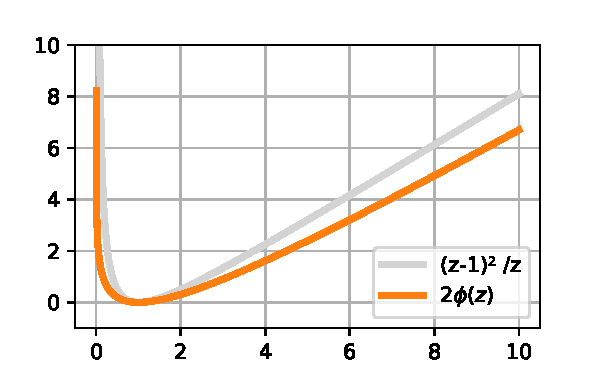
\includegraphics[width=.4\textwidth]{phi.pdf}
	\caption{$\phi(z)$ is the Bregman divergence induced by $-\log(z)$. It is a barrier near $0$. As a result, it is poorly approximated by quadratics, but it admits another upper-bound (in grey).}
	\label{fig:phi}
\end{figure}

For MAP, we get an upper bound thanks to
\begin{align}
	\label{eq:log_bound}
	\phi(z) \leq \phi(z) + \phi(\inv{z}) =  \half (z + \inv{z}) - 1 \; .
\end{align}

\section{PROOFS FOR GAUSSIAN}
\label{app:gaussian}

\section{ASYMPTOTIC DERIVATION}
\label{app:asymptote}

\section{SELF-CONCORDANCE}
\label{app:self-concordant}

\section{TODO}
\begin{enumerate}
	\item new plots : add 2d trajectories to paper, with background level set, and new legend : primal/dual expectation, and clear explanation !
	\item Incorporate related work by Frederik.
	\item Technical Background : be precise and add reference for the steep exponential family of Legendre type which guarantees that our sets are open, and have a solution in the middle.
	References: \begin{itemize}
		\item \href{https://www.jstor.org/stable/4616462?seq=1#metadata_info_tab_contents}{Existence of Maximum Likelihood Estimates for Multi-Dimensional Exponential Families},
		\item The singly truncated normal distribution: A non-steep exponential family,
		\item Statistical exponential families: A digest with flash cards,
		\item Information and Exponential Families In Statistical Theory,
		\item Fundamentals of Statistical Exponential Families with Applications in Statistical Decision Theory.
	\end{itemize}
\end{enumerate}




\section{Blurbs/ideas?}



\subsection{SGD blurb}
\fdk{
%
There is a long line work bounding the convergence rate of stochastic gradient descent.
Beyond the results of \citet{robbins1951stochastic},
we now have proofs on smooth, strongly convex problems and bounded variance
(as well as other assumptions on the noise, reviewed later)
a decreasing step-size and an averaging scheme gets
a $1/t$ convergence rate,
which matches the asymptotic rate of unbiased estimation,
through clever averaging schemes \citep{rakhlin2012making,lacostejulien2012simpler}
\\
Those papers assume the stochastic gradients are bounded,
but small modifications also work for bounded variance instead.
\\
We do have extensions to other notions of bounded variance,
for example assuming that the stochastic gradients are gradients of a perturbed smooth function $f_i$
and that the minimum of $f$ and the minima of the $f_i$
are bounded, $\expect{\min_x f(x) - \min_x f_i(x)} \leq \sigma^2$,
or that the gradient noise is bounded only at the minimum.
For a review, see \citet{gower2019sgd}.
\\
However, for some problems, combining decreasing step-sizes and averaging is not necessary,
even when the function is not strongly convex.
This is the case for maximum likelihood estimation and matches the asymptotic rates,
but holds more generally, for example for linear and logistic regressions \citep{bach2013nonstronglyconvex,moulines2011non}.
}


\subsection{Poisson likelihood?}
\fdk{
\citet{bauschke2017descent} and \citet{hanzely2018fastest} both use the example of Poisson inverse problems/Poisson regression
as examples.
The simpler case of the MLE of a Poisson distribution is also unsolved, though.
In this case, $h(x) = 1/x!$, $x \in \mathbb{N}$, $A(\theta) = e^\theta$ over $\theta \in \mathbb{R}$,
$A^*(\m) = \m \log \m - \m$ over $\m \in \mathbb{R}_+$.
It is neither strongly-convex nor self-concordant (at least according to the standard definition,
although it satisfies generalized notions of self-concordance as $A'''(\theta) = A''(\theta)$).
}

\subsection{``simple'' open problem?}
\fdk{
A ``simple open problem'';
assume we have a deterministic problem, so that we know where the minimum is.
Can we figure out a (deterministic) path from $\theta_0$ to $\theta_*$
that has optimality decreasing as $1/n^2$,
to mirror the bias term of gradient descent?
}

\subsection{Connection with acceleration?}
\fdk{
The problems on how to deal with Bregman divergences abound in optimization, beyond stochasticity.
For example, we haven't yet figured out the analog of Nesterov-type acceleration
on relatively smooth and strongly convex problems,
to bring the convergence rate from linear in $(1-\kappa)$ to $(1-\sqrt{\kappa})$,
or just from $1/T$ to $1/T^2$ in the (non-strongly) convex case.
\citet{dragomir2021optimal}  shows that naïve application of Bregman updates can not achieve acceleration.
The tools developed to make progress on one problem might help make progress on the other.
}






\newpage
\section{Notation convention}
We use
\begin{itemize}
	\item $\theta, \nat$ for natural parameters
	\item $\m$ for mean parameters
	\item $X_1,\ldots,X_n$ for data
	\item $\cX$ for the data space
	\item $T$ for the sufficient statistics
	\item $\nu$ for the base measure
	\item $A, A^*, \logpart, \conj$ for the log-partition and its dual
	\item $\cB_A$ for the Bregman divergence induced by $A$
	\item $n$ for the number of samples
	\item $(\theta^*,m^*)$ for the optimum
	\item $\gamma, \lr$ for the step-size
	\item $\mu,\sigma^2$ for the parameters of a Gaussian
	\item $\hat\theta_n$ for estimates
	\item $\tilde\theta_n$ for $\expect{\hat\theta_n}$, which is biased
	\item $(\stgcvx , \smooth)$ for strong-convexity and smoothness
\end{itemize}

\end{document}